%\setchapterpreamble[u]{}

\chapter{Concept} \label{chap:Concept}
\minitoc\vspace{1em}

\section{Background}
In this chapter, we will present the approaches we used for solving the problem.
First we will focus on the fundamentals of the graph theory. Next we will introduce the notion of similarity and distance, and give some examples. We will conclude this chapter by explaining what association rules are and how to extract information from them. 

\section{Graph Theory Fundamentals}
\subsection{Labeled Graphs}
Graph $G = (V,E)$ is a finite non-empty set of vertices $V = {v_{1}, v_{2}, …}$ with a set of edges $E = {e_{1}, e_{2}, …}$ that connect pairs of vertices.
If the edges have direction, then the $G$ is a directed graph (digraph). 
An ordered pair describes the directionality of an edge $e$ as $e = (u,v)$,
where $u$ is the starting vertex (source) and $v$ is the ending vertex (target). 

A labeled graph $G$ is a graph where vertices or edges are associated with labels \cite{Champin2003}. 
More precise, given a finite set of vertex labels $L_{V}$ and a finite set of edge labels $L_{E}$, a labeled graph is defined by a the tuple $G = (V, E, r_{V} , r_{E})$ such that:

\begin{itemize}
	\item[--]  $V$ is a finite set of vertices,
	\item[--] $r_{V} \subseteq V \times L_{V}$ is the function that assigns labels to vertices
	\item[--]  $r_{E} \subseteq V \times V \times L_{E}$ is the function that assigns labels to edges
\end{itemize}

The tuples from $r_{V}$ and $ r_{E} $ describe the vertex features and edge features of $G$ respectively. 

%For labeled directed graphs, the set of edges is now formally described with additional parameter $l$ that corresponds to the label:
%\begin{equation}
% E = \{(u, v) | \exists l, (u, v, l) \in r_{E}\}
%\end{equation}

\subsection{Node Ranking}
Ranking the nodes (vertices) reflects their importance within a graph. 
Based on the link structure, we estimate how relevant certain node is.
The very straightforward way for computing a rank is the degree of the node: the number of incoming and outgoing  edges from a node. However, this doesn’t propagate the score throughout the nodes.

To overcome this, we use the PageRank (PR) algorithm \cite{PageRank}. PR ranks all the node in a graph by forming a probability distribution i.e.\ the cumulative score of all PR scores sums up to one. 

PR will assign high score to a node if: (1) there are many nodes pointing to it and (2) those nodes also have high PR score.


\begin{equation}
	PR(X) = (1-d) + d(\dfrac{PR(V_{1})}{O(V_{1})} + ... + \dfrac{PR(V_{N})}{O(V_{N})})
\end{equation}
\todo{Explain PR algorithm}

\subsection{Graph Comparison}

Two labeled graphs $G_{1}$ and $G_{2}$ are considered equal if they have the same set of nodes and they are connected in the same way. 
This is also known as \emph{isomorphism}\cite{Wilson:1986:IGT:22577}. 
%Sub-isomorphism checks whether one graph completely contains the other.%
Isomorphic graphs are identical in structure and labeling. 
This results in a very restrictive measure. 
In a given scenario where most but not all edges and vertices are identical,
the graphs will not be considered equal.

Instead, the \emph{Maximum Common Subgraph} can be considered.
This is the largest subgraph $G$ for the input $(G_{1},G_{2})$ 
such that that there exist subgraph isomorphisms from $G$ to $G_{1}$ and from $G$ to $G_{2}$.
In figure \ref{fig:mcs3} the Maximum Common subgraph is shown for the graphs in figure \ref{fig:mcs1} and \ref{fig:mcs2}.

\begin{figure}[t]
	\begin{subfigure}{.3\textwidth}
		\centering
		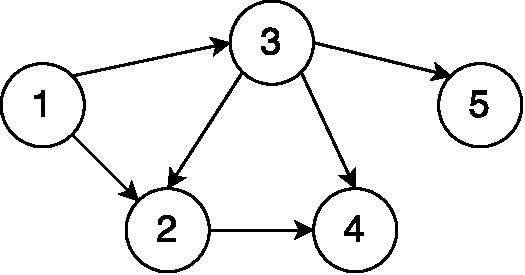
\includegraphics[width=.8\linewidth]{mcs1.pdf}
		\caption{$G_{1}$}
		\label{fig:mcs1}
	\end{subfigure}%
	\begin{subfigure}{.3\textwidth}
		\centering
		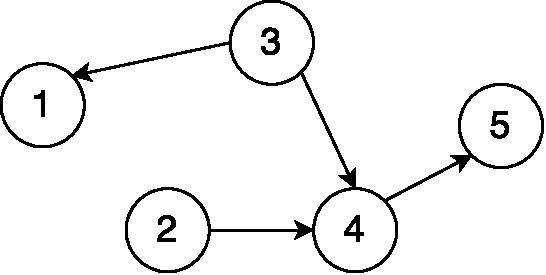
\includegraphics[width=.8\linewidth]{mcs2.pdf}
		\caption{$G_{2}$}
		\label{fig:mcs2}
	\end{subfigure}
\begin{subfigure}{.3\textwidth}
	\centering
	\includegraphics[width=.43\linewidth]{mcs3.pdf}
	\caption{$mcs(G_{1},G_{2})$}
	\label{fig:mcs3}
\end{subfigure}
	\caption{Example of Directed Maximum Common Subgraph for input $(G_{1},G_{2})$ }
	\label{fig:mcs}
\end{figure}
 
 However, it is shown that this evaluation is NP-complete \todo{refer}{\url{https://cise.ufl.edu/class/cot5405sp10/assignments/HW4sol.pdf}}.

\section{Similarity}
\subsection{Introduction}
The concept of similarity appears in almost every scientific domain. 
It is defined by similarity measure (similarity function), based on object representations.
If we consider the following spaces: $\mathds{F}$, which denotes the feature space
and $\mathds{R} ^  \mathds{F}$ - the space of all feature representations,
then the similarity is a mapping from the future space to a score 
$s: \mathds{R}^{\mathds{F}} \times  \mathds{R}^{\mathds{F}} \rightarrow  \mathds{R}$.

In other words, by using similarity as criterion, we can evaluate the likeliness between objects by quantifying how closely related they are.


Similarity function $s$ is subject to the following properties: \cite{Santini:1999:SM:317043.317048}:

\begin{itemize}
	\item[--] Symmetry: $\forall x,y \in \mathds{X}: s(x,y) = s(y,x)$ - the order of the objects in the input should not affect the output score
	\item[--] Maximum self-similarity: $\forall x,y \in \mathds{X}: s(x,x) \geqslant s(x,y)$ - nothing can be more similar than the object itself
\end{itemize}

For applying similarity function, an object representation is needed with a corresponding distance function. 
Object representation allows us to extract the features from the given data objects. 
Depending on the domain, different feature extraction methods can be applied. 

The distance function allows us to give score for the closeness between the corresponding features.
It directly corresponds to the dissimilarity measure: it gets value close to zero for objects which are similar (i.e. close) to each other. 
In other words, similar objects tend to have short distances between one another.

For function $d:\mathds{X} \times \mathds{X} \rightarrow :\mathds{R}$ to qualify as distance, in needs to fulfill the following constraints\cite{Deza.Deza2009EncyclopediaofDistances}:
\begin{itemize}
	\item[--] Non-negativity: $\forall x,y \in \mathds{X}: d(x,y) \leqslant 0$
	\item[--] Reflexivity: $\forall x \in \mathds{X}: d(x,x) = 0$
	\item[--] Symmetry: $\forall x,y \in \mathds{X}: d(x,y) = d(y,x)$
\end{itemize}

Further more, a distance $d$ is a metric, if it additionally satisfies the following properties:
\begin{itemize}
	\item[--] Identity of indiscernibles: $\forall x,y \in \mathds{X}: d(x,y) = 0 \Leftrightarrow x=y$
	\item[--] Triangle inequality: $\forall x,y,z \in \mathds{X}: d(x,y) \leqslant d(x,z) + d(y,z)$
\end{itemize}

\subsubsection{Conversion from Distance to Similarity}

The conversion from distance to similarity may differ. 
Any monotonically decreasing transformation can be applied to convert similarity measures into dissimilarity measures, 
and any monotonically increasing transformation can be applied to convert the similarity to distance.
\todo{Cite lecture notes}{\url{http://users.csc.calpoly.edu/~dekhtyar/560-Fall2009/lectures/lec09.466.pdf}}

If the similarity values are normalized in the range from 0 to 1 (degree of similarity), then the corresponding dissimilarity can be expressed as : 
\begin{equation}
d(x,y) = 1 - s(x,y)
\label{dissim}
\end{equation}

\subsection{Example Distance and Similarity Functions Between Features}
Given two objects from the same set $\forall x,y \in \mathds{X}$ we will list several distance and similarity measures (distance functions are labeled with $d$, where similarity functions with $s$).
\subsubsection{Euclidean distance}

Euclidean distance measures the direct distance between two points in Euclidean space. For two d-dimensional points $x$ and $y$, the Euclidean distance is defined as:
\begin{equation}
	d^{EUC}(x,y) = \sqrt{(x_{1} - y_{1})^{2} + (x_{2} - y_{2})^{2} + ... + (x_{d} - y_{d})^{2} } = \sqrt{\sum_{i=1}^{d} (x_{i}-y_{i})^{2}}
\end{equation}

 \todo{explain} {Norm of the vector}:

\begin{equation}
	\lVert x\lVert = \sqrt{\sum_{i=1}^{d}x_{i}^{2}}
	\title{eq:norm}
\end{equation}

The Euclidean distance is a metric distance\cite{Deza.Deza2009EncyclopediaofDistances}.

\subsubsection{Cosine Similarity}
The cosine similarity is defined through the dot product between vectors. For two vectors $x$ and $y$, the dot product is expressed as:

\begin{equation}
	x\cdot y^{T} = \lVert x\lVert \lVert y\lVert \cos{\theta}
	\label{eq:dot}
\end{equation}


where the $\lVert x\lVert$ and $\lVert y\lVert$ are the norms of the vectors x and y respectively), 
and $\theta$ is the angle between the two vectors.
The equation \ref{eq:dot} can be used to express the $\cos \theta$ value as similarity measure:

\begin{equation}
	\cos \theta = s^{COS}(x,y) = \dfrac{x \cdot y}{\lVert x\lVert \lVert y\lVert} = 
	\dfrac{\sum_{i=1}^{d}x_{i}y_{i}}{\sqrt{\sum_{i=1}^{d} x_{i}^{2}}\sqrt{\sum_{i=1}^{d} y_{i}^{2}}}
	\label{eq:cosine}
\end{equation} 

Equation \ref{eq:cosine} defines the cosine similarity function $s^{COS}$, which combines dot product (nominator) with normalization (denominator).

The cosine similarity looks into the angle between the vectors. 
For $\theta$ values close to zero, the cosine similarity will assign a value close to 1, which means that that the two vectors are very similar to each other. 
Although the cosine value ranges between -1 and 1, if we restrict the features only to positive values as shown in TF-IDF 
\todo{Refer to TF-IDF chapter}, the value of $\theta$ will range from 0 to 90 degrees. 
Consequently, the cosine similarity will range between 0 and 1.

This normalization allows us to define the Cosine distance as 
$d^{COS}=1 - \cos \theta$. 
However, this is not a metric distance, as it does not fulfill the triangle inequality.

\subsubsection{Binary Similarity}
The binary similarity corresponds to exact matching. 

\begin{equation}
s^{BIN}(x,y)=
\begin{cases}
1  & \quad \text{if } x=y \\
0  & \quad \text{else }\\
\end{cases}
\label{eq:binary} 
\end{equation}

Although very restrictive, the binary similarity can be easily applied to any domain. 
 
\subsubsection{Hamming Distance}
The Hamming distance between two strings counts the number of positions where different elements occur:

\begin{equation}
	d^{HAM}(x,y) = \sum_{i=1}^{n}d^{BIN}(x_{i},y_{i}) $$where$$ 
	d^{BIN}(x_{i},y_{i})=
	\begin{cases}
	0  & \quad \text{if } x=y \\
	1  & \quad \text{else }\\
	\end{cases}
\end{equation}
As a constraint, the arrays have to be off the same length. 
This can be easily overcome by counting the empty places in the shorter array. 

Hamming distance relies on very strict matching. This results in failure to recognize sub-array alignment (longest common parts). 
In example at \figref{fig:hamming}, given the strings \emph{"EVALUATION"} and \emph{"REALIZATION"}, 
the Hamming Distance is 9, 
since only the substring \emph{"AL"} occurs at the same position at the two inputs.

\begin{figure}[ht]
	\centering
	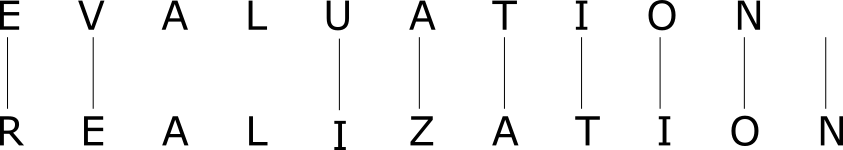
\includegraphics[width=0.7\textwidth]{hamming.png}
	\caption{Hamming Distance Example} 
	\label{fig:hamming}
\end{figure}

\subsubsection{Edit Distance}
The Edit Distance  is a measure for quantifying the dissimilarity between two vectors\cite{Jurafsky:2009:SLP:1214993}.
It is also known as \emph{Levenshtein Distance}, which was specifically defined for string comparison 
(also referred as \emph{String Edit Distance})\cite{Navarro:2001:GTA:375360.375365}.

The (String) Edit distance equals the number of operations required to transform array $x$ into array $y$. 
This operations are limited to:
\begin{itemize}
	\item[--] Insertion of single character
	\item[--] Substitution of single character
	\item[--] Deletion of single character
\end{itemize}

The formal expression of is given with equation \ref{eq:edit-distance}.
\begin{equation}
	d^{EDIT}(x,y) = 	
	\begin{cases}
	size(x)	  & \quad \text{if } size(y)=0 \\
	size(y)	  & \quad \text{if } size(x)=0 \\
	d^{EDIT}(start(x),start(y))	  & \quad \text{if } last(x)=last(y) \\
	1 + min\begin{cases}
		d^{EDIT}(start(x),start(y)),
		d^{EDIT}(start(x),y), \\
		d^{EDIT}(x,start(y)) \\
		\end{cases} & \quad \text{else }\\
	\end{cases} 
	\label{eq:edit-distance}
\end{equation}

Edit Distance overcomes the drawbacks of the Hamming Distance. 
It is robust in terms of substrings alignment. 
This can be shown on the given strings are \emph{"EVALUATION"} and \emph{"REALIZATION"} in \figref{fig:edit}.
These common substrings remain unmodified. 
The remaining operations needed to convert string X to Y are:
\begin{itemize}
	\item[--] One insertion of character 'R'
	\item[--] One deletion of character 'V'
	\item[--] One insertion of character 'I'
	\item[--] One substitution of character 'U' to 'Z'
\end{itemize}

\begin{figure}[ht]
	\centering
	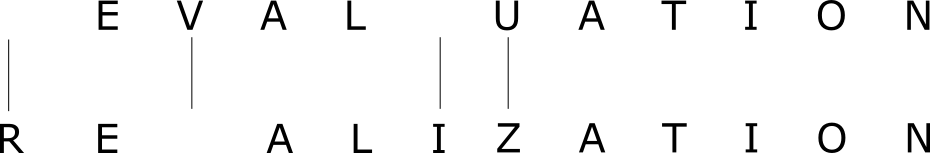
\includegraphics[width=0.7\textwidth]{edit.png}
	\caption{Edit Distance Example} 
	\label{fig:edit}
\end{figure}
This results in total of 4 operation, giving the distance (or cost) of 4.

Assigning cost to each operation results into Weighted Edit Distance\cite{Chen:2004:MLE:1316689.1316758}.

Both Edit Distance and the Weighted Edit Distance are metric.

\subsection{Example Distance and Similarity Functions Using Graph Structure}

\subsubsection{Neighborhood Random Walk Distance}

Based on the connectivity in a graph $G$, a distance measure between vertices can be defined. 
Two nodes $v_{a}$ and $v_{b}$ are considered close if there are multiple paths connecting them. 
If there are few or no paths, then the are considered dissimilar.

\begin{definition}
	Given $l$ as the upper bound how far a random walker can go and the restart probability $c \in [0, 1]$, 
the Random Walk Distance between two nodes  $x$ and $y$ in graph $G$ is defined as:
\begin{equation}
	d^{NRW}(x,y) = \sum_{\tau:v_{i}\rightsquigarrow v_{j}}p(\tau)c(1-c)^{len(\tau)}
\end{equation}
defined for all paths $\tau$ between $v_{a}$ and $v_{b}$ whose length is shorter than $l$ with transition probability p($\tau$). 
\end{definition}

For unweighted graph, the probability distribution of edges considered in the final path is uniform.

\subsubsection{SimRank}
SimRank calculates similarities between vertices in graph $G$ based on their structural context\cite{Jeh02simrank:a}.
The underlying idea of this algorithm is that two objects are similar if they are referenced by similar other objects. 
The objects are modeled as vertices (nodes) and the relations between them as directed edges.
This makes SimRank domain independent, applicable for every domain that can be modeled using the basic directed graph model.

Formally, SimRank is expressed in \ref{eq:simrank}.
\begin{equation}
	s^{SR}(x,y) = \dfrac{C}{\arrowvert I(x)\arrowvert \arrowvert I(y)\arrowvert}
	\sum_{i=1}^{\arrowvert I(x)\arrowvert}
	\sum_{j=1}^{\arrowvert I(y)\arrowvert}s^{SR}(I_{i}(x), I_{j}(y))
	\label{eq:simrank}
\end{equation}
The constant $C \in [0,1]$ is a user given factor for decay, $I(v)$ is the set of predecessor nodes for a given node $v$, 
and $\arrowvert I(v)\arrowvert$ is the size of that set.
Dividing by the total number of predecessors pairs allows us to obtain normalized value: 
a range between 0 (maximum dissimilarity) to 1 (same pair of nodes). 

For veticies that have no predecessors ($I(v)=\emptyset$), the similarity is set to zero.
Alternatively, equation \ref{eq:simrank} can be expressed using the set of successors $O(v))$ of the node $v$,
or combining the result from both approaches.

As stated, the intuition behind this approach is recursive - 
in order to define similarity between two objects, we need to rely on already pre-calculated similarity between the neighbors.
SimRank is computing by iteratively evaluating over each pair of nodes $(v_{a},v_{b})$ until fixpoint is reached. 
The initial similarity score is  calculated using the binary similarity (equation \ref{eq:binary}):

\begin{equation}
	s_{0}^{SR}(v_{a},v_{b}) = \begin{cases}
	1  & \quad \text{if } v_{a}=v_{b} \\
	0  & \quad \text{else }\\
	\end{cases}
\end{equation}
The node pairs, where the $s_{0}^{SR}(v_{a},v_{b})=1$ are called singleton pairs.
For each iteration $k$, the similarity score $s_{k+1}^{SR}$ is updated using $s_{k+1}^{SR}$:

\begin{equation}
	s_{k+1}^{SR}(v_{a},v_{b})= \dfrac{C}{\arrowvert I(v_{a})\arrowvert \arrowvert I(v_{b})\arrowvert}
	\sum_{i=1}^{\arrowvert I(v_{a})\arrowvert}\sum_{j=1}^{\arrowvert I(v_{b})}s_{k}^{SR}(I_{i}(v_{a}), I_{j}(v_{b}))
\end{equation}
where $v_{a}\neq v_{b}$ (we only update the score for non-singleton pairs).

The end result after $K$ iterations is a graph $G^{2} = (V^{2},E^{2})$, where the nodes are pairs from $G$
and the edges are aggregated for both elements of the vertex pair:
\begin{itemize}
	\item[--] $V^{2} = V\times V$ are vertex pairs in $V$
	\item[--] $E^{2}:(a,b) \rightarrow (c,d)$ in $G^{2}$ iff $a\rightarrow c$ and $b\rightarrow d$ in $G$
\end{itemize}
Example is given in figure \ref{fig:simrank}. For the input \ref{fig:simrank1}, SimRank outputs the $G^{2}$ as showed on \ref{fig:simrank2}, using the decay factor $C=0.8$.

\begin{figure}[t]
	\begin{subfigure}{.35\textwidth}
		\centering
		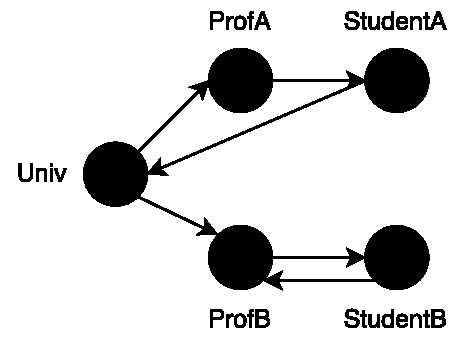
\includegraphics[width=.8\linewidth]{simRank1.pdf}
		\caption{$G$}
		\label{fig:simrank1}
	\end{subfigure}%
	\begin{subfigure}{.65\textwidth}
		\centering
		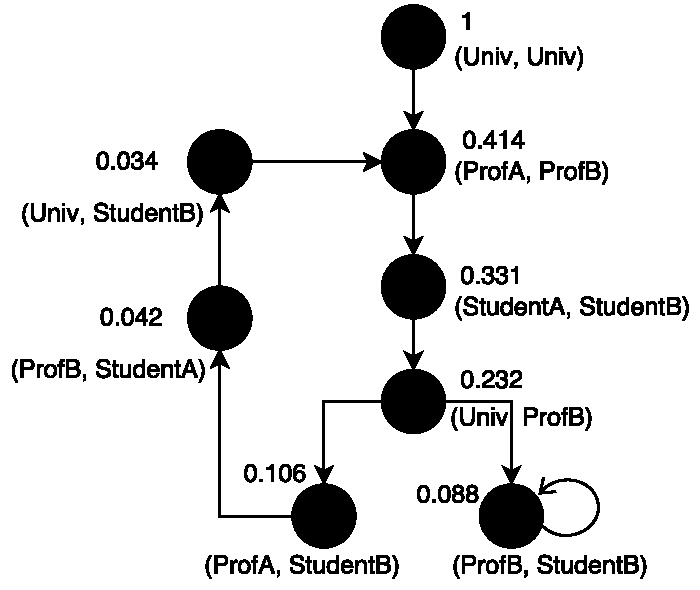
\includegraphics[width=.8\linewidth]{simRank2.pdf}
		\caption{$G^{2}$}
		\label{fig:simrank2}
	\end{subfigure}
	\caption{Example of SimRank on Directed Maximum Common Subgraph for input $(G_{1},G_{2})$ }
	\label{fig:simrank}
\end{figure}

\section{Association Analysis}
Association rule mining searches for recurring relationships in dataset.
More specific, it discovers the associations and correlations among items\cite{Han:2005:DMC:1076797}.
\subsection{Definition}
Let $I=\{I1,I2,..,Im\}$ be n set of one or more items (also referred as itemset).
An itemset of length k is labeled as k--itemset.

Let $D$ be the database of transactions where each transaction is a non-empty itemset such that $T \subseteq I$.
Transaction $T$ is said to contain an itemset $A$  if $A\subseteq T$.
The goal of association rule mining is given the set of transactions $T$, 
find association rules that will predict the occurrence of an item $I$ based on the occurrences of other items in the transaction $T$.

An association rule indicated as 
$\{A_{1},A_{2},...,A_{m}\}\Rightarrow \{B_{1},B_{2},...,B_{n}\}$, 
where $\forall i,j \mid i\leq m,j\leq n$, $A_{i}$ and $B_{j}$ are non-empty itemsets. This indicates that if the transaction $T$ contains items $A_{1},..A_{m}$, it is highly likely that the items $B_{1},...,B_{m}$ would be of interest of $T$.
\subsection{Association Rule Interestingness }
For evaluating the interesting of rules, the \emph{support} and \emph{confidence} metrics are used.
Support $supp$ for the rule $A\Rightarrow B$ indicates the fraction of transactions that contain both $A$ and $B$:
\begin{equation}
	supp(A\Rightarrow B) = P(A\cup B)
\end{equation}
Support will filter out rules that occurred by chance.
%A rule with support above a given \emph{minimum support} threshold ($minsup$) is %called \emph{frequent itemset}.
Confidence $conf$ for the rule $A\Rightarrow B$ indicates the fraction of items contained in $B$ that are also contained in $A$.
\begin{equation}
	conf(A \Rightarrow B) = P(B|A)
\end{equation}
Confidence measures the reliability made by a rule.

Rule with support $\geq minsup$ and $conf\geq minconf$,
where $minsup$ and $minconf$ are user defined thresholds,
are called \emph{strong rules}.
	
\subsection{Association Rule Mining}

Association rule mining is performed in two steps:
\begin{enumerate}
	\item Frequent itemset generation i.e.\ itemsets with support $\geq minsup$
	\item Strong rules generation from the frequent itemsets 
\end{enumerate}

\subsubsection{Generating Frequent Itemsets}

Using na\"{\i}ve approach, we count the frequency of all possible subsets in the database. 
That means match each transaction against every candidate. 
Although this would work, the number of itemsets rises exponentially
If $m$ is the total number of given items, the number of candidates for frequent itemset will be $2^{m}$\cite{Han:2005:DMC:1076797}.

Instead of evaluating all the possible combinations, 
the Apriori algorithm\cite{Agrawal:1994:FAM:645920.672836} uses the principle of anti monotonicity to prune the generation of candidates: 
if an itemset is frequent, then all of its subsets must also be frequent.
If an item $I$ does not satisfy the $minsup$ threshold (not frequent item),
then it is not of our interest - since adding new item $A$ to this itemset cannot occur more frequently than $minsip$. 
This means that $P(I \cup A)$ < $minsup$, so we don’t need to consider additional items for $I$. 
The algorithm first counts the 1--itemsets, then the 2-itemsets and iteratively increases the k--itemset size until no more candidates are generated.
Each iteration consists of two steps: join and prune. 
In the join step, the list of candidates $C_{k+1}$ is generated by joining the previous list of candidates $ C_{k} $ with itself. 
In the prune step, all the k--itemsets that are infrequent are removed.
After the list of frequent itemsets is obtained, generating the strong rules is done by filtering out all the rules below the confidence threshold.

\makeatletter
\def\BState{\State\hskip-\ALG@thistlm}
%\makeatother
\begin{algorithm}
	\caption{Apriori}\label{}
	\begin{algorithmic}[1]
		\Procedure{Apriori}{T,$minsup$}			
			\BState $k \gets 1$
			\BState $L_{k} \gets \{$\textit{all 1--temsets}$\}$
			\BState {\textbf{repeat}}:
			\State $C_{k+1}  \gets \textit{GENCANDIDATES}(L_{k})$
			\For {\textbf{each} \textit{transaction t}}
				\State \textit{increment the count of candidates in }$C_{k+1}$
					   \texit{ contained in }$T$
				\State  $L_{k+1}=\textit{candidates in }C_{k+1} \textit{with supp} \geq minsup$
			\EndFor
			\BState \textbf{until} $L_{k} \neq \emptyset$ \\
			\Return $\cup_{k}L_{k}$
		\EndProcedure
		
		\Procedure{gencandidates}{$L_{k}$}
			\State $C_{k+1} \gets \textit{join}(L_{k},L_{k})$
			\For{\textbf{all}\textit{ itemsets }$c$\textbf{ in } $C_{k+1}$}
				\For{\textbf{all}\textit{ k--itemsets }$s$\textbf{ of } $c$}
					\If{$s$ \textit{ not in } $L_{k}$}
						{\textbf{ delete }$c$ \textbf{ from }$C_{k+1}$}
					\EndIf
				\EndFor
			\EndFor
			\\\Return $C_{k+1}$
		\EndProcedure
	\end{algorithmic}
\end{algorithm}

\subsubsection{Correlation Analysis}
Minimum support and confidence is shown to be misleading\cite{Lin:2002:CSS:646420.693806}.To avoid this, an additional measure of correlation can be used to evaluate rules:\ $A\Rightarrow B [support, confidence, correlation]$. 
\textbf{Lift} is a simple correlation measure which compares the likelihood of the both items belong to the same transaction versus the likelihood of the two items belonging to two different transactions\ref{eq:lift}:  
\begin{equation}
	lift(A,B) = \frac{P(A\cup B)}{P(A)P(B)}
	\label{eq:lift}
\end{equation}
If the $lift(A,B) > 1$ then $A$ and $B$ are positively correlated,
if the $lift(A,B) < 1$ then they are negatively correlated, 
and if the lift value equals to 1  then they have no correlation. 

